\documentclass[nobib]{tufte-handout}
\usepackage{amro-common}
\usepackage{amro-tufte}

\newcommand{\cpp}{C\texttt{++}}

% Might prevent marginnotes from jumping to another page
\def\mathnote#1{%
  \tag*{\rlap{\hspace\marginparsep\smash{\parbox[t]{\marginparwidth}{%
  \footnotesize#1}}}}
}


% % This command is needed for building in linux
% \captionsetup{compatibility=false}

\newcommand{\lplus}{\overset{{\scriptscriptstyle\mathrm{L}}}{\oplus}}
\newcommand{\liplus}{\overset{{\scriptscriptstyle\mathrm{LI}}}{\oplus}}
\newcommand{\rplus}{\overset{{\scriptscriptstyle\mathrm{R}}}{\oplus}}
\newcommand{\riplus}{\overset{{\scriptscriptstyle\mathrm{RI}}}{\oplus}}
% Ominus
\newcommand{\lminus}{\overset{{\scriptscriptstyle\mathrm{L}}}{\ominus}}
\newcommand{\liminus}{\overset{{\scriptscriptstyle\mathrm{LI}}}{\ominus}}
\newcommand{\rminus}{\overset{{\scriptscriptstyle\mathrm{R}}}{\ominus}}
\newcommand{\riminus}{\overset{{\scriptscriptstyle\mathrm{RI}}}{\ominus}}



\title{Filtering in C++}
\author{Amro Al~Baali}

% Generates the index
\usepackage{makeidx}
\makeindex

\setcounter{tocdepth}{2}


\begin{document}
    % \frontmatter
    {    
        \makeatletter
\begin{titlepage}
    \begin{fullwidth}    
        \begin{center}
            
            % \vspace*{cm}
                
            % % \includegraphics[width=0.3\textwidth]{figs/McGill_Wordmark.png}
            % \vspace{0.5cm}
            
            % \Huge
            % \textsc{McGill University}
            % \vspace{0.5cm}
            
            % \Huge
            % \textsc{DECAR Group}
            
            % \vspace{0.5cm}
            
            \LARGE
            \textsc{Notes}
            
            \vspace{5cm}
            
            \Huge
            % \thline
            \vspace{0.6em}
            \textbf{\@title}
            % \thline
            
            \vfill
            
            \Large
            {\@author}\\[10pt]
            % 26062940\\[10pt]
            % \textit{Supervisor:}\\
            % {Prof.} {James Richard Forbes}\\[10pt]
            

            % \large
            % Department of Mechanical Engineering, McGill University\\
            % 817 Sherbrooke Street West, Montreal, QC, H3A 0C3\\[10pt]
            
            \today
            
        \end{center}    
    \end{fullwidth}
\end{titlepage}
        % \forceheader{Contents}
        \tableofcontents
        \clearpage
        % \thispagestyle{empty}
        % \addtocontents{toc}{\protect\thispagestyle{empty}}
    }
    % \mainmatter

    \section{Why this document?}
    This document is provided to explain and clarify the code uploaded with it. The repository includes examples of implementing filters, usually Kalman fitlers, in \cpp. The filters will be mainly implemented on 
    \begin{enumerate}
        \item a linear system, and
        \item a non-Euclidean nonlinear system (usually defined on a Lie group).
    \end{enumerate}

    \section{The Kalman filter}
    \subsection{The system}
    Consider the linear ordinary differential equation (ODE) describing a mass-spring-damper system
    \begin{align}
        \label{eq:mass spring damper ode}
        m\ddot{x}(t) + b\dot{x}(t) + kx(t) &= u(t),
    \end{align}
    where $m$ is the mass, $b$ is the damping, $k$ is the spring constant, and $u(t)$ is the forcing function. The system \eqref{eq:mass spring damper ode} can be written in state space form
    \begin{align}
        \mbfdot{x} &= \bbm 0 & 1\\ -\f{k}{m} & -\f{b}{m} \ebm \mbf{x} + \bbm 0\\\f{1}{m} \ebm u\\
        &= \boldsymbol{A}\mbf{x} + \boldsymbol{B}u_{t},
    \end{align}
    where 
    \begin{align}
        \label{eq:DT linear kinematic model}
        \mbf{x} &= \bbm x & \dot{x} \ebm^{\trans},
    \end{align}
    and the time arguments $(t)$ are dropped for brevity.

    The disrete-time kinematic model is given by
    \begin{align}
        \mbf{x}_{k} &= \mbf{A}\mbf{x}_{k-1} + \mbf{B}u_{k-1},        
    \end{align}
    where the discrete-time system matrices $\mbf{A}$ and $\mbf{B}$ are computed using some discretization scheme. For the linear example above, the $\mbf{A}$ matrix is given by
    \begin{align}
        \mbf{A} &= \exp\left( \boldsymbol{A} T_{k} \right),\\
        \mbf{B} &= \int_{0}^{T_{k}}\exp(\boldsymbol{A}\alpha)\dee\alpha \boldsymbol{B},
    \end{align}
    where $T_{k}$ is the sampling period \cite{Farrell_Aided_2008}.
     
    The matrix $\mbf{B}$ can be approximated using forward Euler to get
    \begin{align}
        \mbf{B} &\approx T_{k}\boldsymbol{B}.
    \end{align}

    \subsection{Process model}
    The discrete-time process model\sidenote{Also referred to as the kinematic model, motion model, progression model, \etc.} is used in the \emph{prediction} step of the Kalman filter. It is given by
    \begin{align}
        \label{eq:DT linear process model}
        \mbf{x}_{k} &= \mbf{A}\mbf{x}_{k-1} + \mbf{B}\mbf{u}_{k-1} + \mbf{L}\mbf{w}_{k-1},
    \end{align}
    where $\mbf{x}_{k}\in\rnums^{n_{x}}$ is the state, $\mbf{u}_{k}\in\rnums^{n_{u}}$ is the control input, and $\mbf{w}_{k}\in\rnums^{n_{w}}$ where $\mbf{w}_{k}\sim\mc{N}\left( \mbf{0}, \mbf{Q}_{k} \right)$ is the process noise and $\mbf{Q}_{k}$ is the process noise covariance. 

    \subsection{Measurement functions}
    The correction step requires a measurement model which is given by
    \begin{align}
        \mbf{y}_{k} &= \mbf{C}\mbf{x}_{k} + \mbf{M}\mbf{n}_{k},
    \end{align}
    where $\mbf{y}_{k}\in\rnums^{n_{y}}$ and $\mbf{n}_{k}\in\rnums^{n_{n}}$ where $\mbf{n}_{k}\sim\mc{N}\left( \mbf{0}, \mbf{R}_{k} \right)$ is the measurement noise and $\mbf{R}_{k}$ is the measurement noise covariance.

    For the example presented, the measurement is a position measurememnt, so the measurement function is given by
    \begin{align}
        y_{k} &= \bbm 1 & 0 \ebm\mbf{x}_{k} + n_{k}\\
        &= \mbf{C}\mbf{x}_{k} + n_{k}.
    \end{align}


    %%%%%%%%%%%%%%%%%%%%%%%%%%%%%%%%%%%%%%%%%%%%%%%%%%%%%%%%%%%%%%%%%%
    % EKF
    %%%%%%%%%%%%%%%%%%%%%%%%%%%%%%%%%%%%%%%%%%%%%%%%%%%%%%%%%%%%%%%%%%
    \section{The extended Kalman filter}
    Without getting into the derivation of the equations, the (extended) Kalman filter equations are given by \cite[eq.~(4.32)]{Barfoot_State_2017a}
    \begin{subequations}    
        \label{eq:EKF eqns}
        \begin{align}
            \label{eq:EKF: prediction}
            \mbfcheck{x}_{k} &= \mbf{f}\left( \mbfhat{x}_{k-1}, \mbf{u}_{k-1}, \mbf{0} \right), \\
            \label{eq:EKF: prediction cov}
            \mbfcheck{P}_{k} &= \mbf{A}_{k-1}\mbfhat{P}_{k-1}\mbf{A}_{k-1}^{\trans} + \mbf{L}_{k-1}\mbf{Q}_{k}\mbf{L}_{k-1}^{\trans},\\
            \label{eq:EKF: KF gain}
            \mbf{K}_{k} &= \mbfcheck{P}_{k}\mbf{H}_{k}\left( \mbf{H}_{k}\mbfcheck{P}_{k}\mbf{H}_{k}^{\trans} + \mbf{M}_{k}\mbf{R}_{k}\mbf{M}_{k}^{\trans} \right)\inv,\\
            \label{eq:EKF: correction}
            \mbfhat{x}_{k} &= \mbfcheck{x}_{k} + \mbf{K}_{k}\left( \mbf{y}_{k} - \mbf{g}_{k}\left( \mbfcheck{x}_{k}, \mbf{0} \right) \right),\\
            \label{eq:EKF: correction cov}
            \mbfhat{P}_{k} &= \left( \eye - \mbf{K}_{k}\mbf{H}_{k} \right)\mbfcheck{P}_{k}\left( \eye - \mbf{K}_{k}\mbf{H}_{k} \right)^{\trans} \nonumber\\&\qquad+ \mbf{K}_{k}\mbf{M}_{k}\mbf{R}_{k}\mbf{M}_{k}^{\trans}\mbf{K}_{k}^{\trans},
        \end{align}
    \end{subequations}
    where 
    \begin{align}
        \mbf{A}_{k-1} &= \left.\pd{\mbf{f}\left( \mbf{x}_{k-1}, \mbf{u}_{k-1}, \mbf{w}_{k-1} \right)}{\mbf{x}_{k-1}}\right|_{\overset{\mbf{x}_{k-1}=\mbfhat{x}_{k-1},}{\mbf{w}_{k-1}=\mbf{0}}},\\
        \mbf{L}_{k-1} &= \left.\pd{\mbf{f}\left( \mbf{x}_{k-1}, \mbf{u}_{k-1}, \mbf{w}_{k-1} \right)}{\mbf{w}_{k-1}}\right|_{\overset{\mbf{x}_{k-1}=\mbfhat{x}_{k-1},}{\mbf{w}_{k-1}=\mbf{0}}},\\
        \mbf{H}_{k-1} &= \left.\pd{\mbf{g}\left( \mbf{x}_{k}, \mbf{n}_{k} \right)}{\mbf{x}_{k}}\right|_{\overset{\mbf{x}_{k}=\mbfcheck{x}_{k},}{\mbf{n}_{k}=\mbf{0}}},\\
        \mbf{M}_{k-1} &= \left.\pd{\mbf{g}\left( \mbf{x}_{k}, \mbf{n}_{k} \right)}{\mbf{n}_{k}}\right|_{\overset{\mbf{x}_{k}=\mbfcheck{x}_{k},}{\mbf{n}_{k}=\mbf{0}}}.
    \end{align}

    The covariance equations \eqref{eq:EKF: prediction cov} and \eqref{eq:EKF: correction cov} are computed using first-order covariance propagation on \eqref{eq:EKF: prediction} and \eqref{eq:EKF: correction}, respectively. Let's clarify this point as it will be important when discussing the invariant extended Kalman filter.

    \begin{remark}    
        \label{remark:splitting gaussian rv into sum}
        A Gaussian random variable 
        \begin{align}
            \mbfrv{x}\sim\mc{N}\left( \mbs{\mu}, \mbs{\Sigma} \right)
        \end{align}
        can be written as
        \begin{align}
            \mbfrv{x} &= \mbs{\mu} + \delta\mbfrv{x},\\
            \delta\mbfrv{x} &\sim \mc{N}\left( \mbf{0}, \mbs{\Sigma} \right).
        \end{align}
    \end{remark}
    Using Remark~\ref{remark:splitting gaussian rv into sum}, define the (random) variables
    \begin{align}
        \label{eq:KF: prediction err. def.}
        \delta\mbfcheckrv{x}_{k} &\coloneqq \mbfcheckrv{x}_{k} -  \mbf{x}_{k},\\
        \label{eq:KF: correction err. def.}
        \delta\mbfhatrv{x}_{k} &\coloneqq \mbfhatrv{x}_{k} -  \mbf{x}_{k},
    \end{align}
    where
    \begin{align}
        \delta\mbfcheckrv{x}_{k} &\sim\mc{N}\left( \mbf{0}, \mbfcheck{P}_{k} \right),\\
        \delta\mbfhatrv{x}_{k} &\sim\mc{N}\left( \mbf{0}, \mbfhat{P}_{k} \right).
    \end{align}
    Using Taylor's expansion of \eqref{eq:EKF: prediction}, the error dynamics of the (extended) Kalman filter equations are then given by
    \begin{align}
        \delta\mbfcheckrv{x}_{k} 
        &= \mbfcheckrv{x}_{k} - \mbf{x}_{k} \\
        &= \mbf{f}\left( \mbfhatrv{x}_{k-1}, \mbf{u}_{k-1}, \mbf{0} \right) - \mbf{f}\left( \mbf{x}_{k-1}, \mbf{u}_{k-1}, \mbfrv{w}_{k-1} \right)\\
        &\approx \mbf{f}\left( \mbfhat{x}_{k-1}, \mbf{u}_{k-1}, \mbf{0} \right) - \mbf{f}\left( \mbfhat{x}_{k-1},\mbf{u}_{k-1}, \mbf{0} \right) 
            \nonumber\\&\qquad
            - \mbf{A}_{k-1}\underbrace{\left( \mbf{x}_{k-1} - \mbfhatrv{x}_{k-1} \right)}_{-\delta\mbfhatrv{x}_{k-1}} - \mbf{L}_{k-1}\left( \mbfrv{w}_{k-1} - \mbf{0} \right)\\
        &= \mbf{A}_{k-1}\delta\mbfhatrv{x}_{k-1} - \mbf{L}_{k-1}\mbfrv{w}_{k-1}.
    \end{align}
    The covariance on $\delta\mbfcheck{x}_{k}$ is then given by
    \begin{align}
        \cov{\delta\mbfcheckrv{x}_{k}} &= \mbf{A}_{k}\mbfhat{P}_{k-1}\mbf{A}_{k-1}^{\trans} + \mbf{L}_{k-1}\mbf{Q}_{k-1}\mbf{L}_{k-1}^{\trans}
    \end{align}
    which is equivalent to \eqref{eq:EKF: prediction cov}.

    Applying the same concept on the correction equation gives
    \begin{align}
        \delta\mbfhatrv{x}_{k} 
        &= \mbfcheckrv{x}_{k} + \mbf{K}_{k}\left( \mbfrv{y}_{k} - \mbf{g}\left( \mbfcheckrv{x}_{k}, \mbf{0} \right) \right) - \mbf{x}_{k}\\
        &= \mbfcheckrv{x}_{k} + \mbf{K}_{k}\left( \mbf{g}\left( \mbf{x}_{k},\mbfrv{n}_{k} \right) - \mbf{g}\left( \mbfcheckrv{x}_{k}, \mbf{0} \right) \right) - \mbf{x}_{k}\\
        &= \mbf{x}_{k} + \delta\mbfcheckrv{x}_{k} + \mbf{K}_{k}\left( \mbf{g}\left( \mbf{x}_{k},\mbfrv{n}_{k} \right) - \mbf{g}\left( \mbfcheckrv{x}_{k}, \mbf{0} \right) \right)\\
        &\approx \delta\mbfcheckrv{x}_{k} +\mbf{K}_{k}\left( \mbf{g}\left( \mbfcheck{x}_{k}, \mbf{0} \right) + \mbf{H}_{k}\left( \mbf{x}_{k} - \mbfcheckrv{x}_{k} \right) \right.\nonumber\\&\qquad \left.+ \mbf{L}_{k}\left( \mbfrv{n}_{k}-\mbf{0} \right) - \mbf{g}\left( \mbfcheck{x}_{k},\mbf{0} \right) \right)\\
        &= \delta\mbfcheckrv{x}_{k} +\mbf{K}_{k}\left( \mbf{H}_{k}\left( \mbf{x}_{k} - \mbfcheckrv{x}_{k} \right) + \mbf{L}_{k}\left( \mbfrv{n}_{k}-\mbf{0} \right) \right)\\
        &= \delta\mbfcheckrv{x}_{k} +\mbf{K}_{k}\left( -\mbf{H}_{k}\delta\mbfcheckrv{x}_{k} + \mbf{L}_{k}\left( \mbfrv{n}_{k}-\mbf{0} \right) \right)\\
        &= \left( \eye - \mbf{K}_{k}\mbf{H}_{k} \right)\delta\mbfcheckrv{x}_{k} + \mbf{K}_{k}\mbf{M}_{k}\mbfrv{n}_{k}.
    \end{align}
    The covariance is then given by
    \begin{align}
        \cov{\delta\mbfhatrv{x}_{k}} &= \left( \eye - \mbf{K}_{k}\mbf{H}_{k} \right)\mbfcheck{P}_{k}\left( \eye - \mbf{K}_{k}\mbf{H}_{k} \right)^{\trans} + \mbf{K}_{k}\mbf{M}_{k}\mbf{R}_{k}\mbf{M}_{k}^{\trans}\mbf{K}_{k}^{\trans}
    \end{align}
    which is equivalent to \eqref{eq:EKF: correction cov}.

    %%%%%%%%%%%%%%%%%%%%%%%%%%%%%%%%%%%%%%%%%%%%%%%%%%%%%%%%%%%%%%%%%%
    % InEKF
    %%%%%%%%%%%%%%%%%%%%%%%%%%%%%%%%%%%%%%%%%%%%%%%%%%%%%%%%%%%%%%%%%%
    \section{The invariant extended Kalman filter}
    The invariant filter\cite{Barrau_Invariant_2018} is applicable to states that live in Lie groups. However, since the filter deals with random variables, it's important to know how to represent random variables living in Lie groups. That is, $\mbfrv{X}\in G$, where $G$ is some group.

    Let the $SE(n)$ process model be given by
    \begin{align}
        \label{eq:InEKF: process model}
        \mbfrv{X}_{k} &= \mbf{F}\left( \mbfrv{X}_{k-1}, \mbf{u}_{k-1}, \mbfrv{w}_{k-1} \right)\\
        &= \mbfrv{X}_{k-1}\Exp\left( T_{k-1}\mbf{u}_{k-1} \right)\Exp(\mbfrv{w}_{k-1})\\
        \label{eq:InEKF: SE3 process model}
        &= \mbfrv{X}_{k-1}\mbs{\Xi}_{k-1}\Exp(\mbfrv{w}_{k-1}),
    \end{align}
    \marginnote[-4em]{$T_{k-1} \coloneqq t_{k}-t_{k-1}$ is the sampling period.}
    the left-invariant measurement model is given by
    \begin{align}
        \label{eq:InEKF: LI meas. model}
        \mbfrv{y}_{k} &= \mbfrv{X}_{k}\mbf{b} + \mbfrv{n}_{k},
    \end{align}
    and the right-invariant measurement model is given by
    \begin{align}
        \label{eq:InEKF: RI meas. model}
        \mbfrv{y}_{k} &= \mbfrv{X}_{k}\inv\mbf{b} + \mbfrv{n}_{k},
    \end{align}
    where $\mbf{b}$ is some known constant column matrix.

    \subsection{Random variables on Lie groups}
    In the Euclidean case, Remark~\ref{remark:splitting gaussian rv into sum} can be used to describe a random variable. However, how can we do that in a non-Euclidean case? Let's restrict ourselves with Lie groups. 
     
    
    A random variable (on a Lie group) can be given by
    \begin{align}
        \mbfrv{X} &= \mbfbar{X}\delta\mbfrv{X}\\
        &= \mbfbar{X}\exp\left( \mbsrv{\xi}\expand \right)\\
        &= \mbfbar{X} \rplus \mbsrv{\xi},
    \end{align}
    where $\rplus$ is the `right perturbation' operator\footnote{There are multiple versions of the $\oplus$ operator such as left, left-invariant, right, and right-invariant.} from
     \cite{Sola_micro_2019} and
    \begin{align}
        \mbsrv{\xi} &\sim \mc{N}\left( \mbf{0}, \mbs{\Sigma} \right).
    \end{align}
    This is the Lie-group version of Remark~\ref{remark:splitting gaussian rv into sum}. Note that $\mbfbar{X}\in G$ and $\exp\left( \mbsrv{\xi}\expand \right)\in G$, thus $\mbfrv{X}\in G$ since $G$ is a Lie group which is closed under multiplication.

    \subsection{Left-invariant perturbation}
    The left-invariant ``addition'' $\liplus : G \times \rnums^{n} \to G$ is defined by
    \begin{align}
        \mbf{X}\liplus\mbs{\xi} 
        &\coloneqq \mbf{X}\exp\left( -\mbs{\xi}\expand \right)\\
        &= \mbf{X}\Exp\left( -\mbs{\xi} \right),
    \end{align}
    and the left-invariant ``subtraction'' $\liminus : G \times G \to \rnums^{n}$ is defined by
    \begin{align}
        \mbf{X}_{2}\ominus\mbf{X}_{1} 
        &\coloneqq \log\left(\mbf{X}_{2}\inv\mbf{X}_{1}\right)\contract\\
        &= \Log\left(\mbf{X}_{2}\inv\mbf{X}_{1}\right).
    \end{align}

    \subsection{The invariant extended Kalman filter}
    Without deep derivation, let's take the extended Kalman filter equations \eqref{eq:EKF eqns} and expand them to states that live on smooth manifolds. Let's simply replace the Euclidean $+$ and $-$ operators with $\oplus$ and $\ominus$, respectively\footnote{There are different `flavors' as discussed above.}. 
    
    The prediction equations will then be
    \begin{align}
        \label{eq:InEKF: state prediction}
        \mbfcheck{X}_{k} &= \mbf{F}\left( \mbfhat{X}_{k-1}, \mbf{u}_{k-1}, \mbf{0} \right),\\
        \label{eq:InEKF: state prediction cov.}
        \mbfcheck{P}_{k} &= \mbf{A}_{k-1}\mbfhat{P}_{k-1}\mbf{A}_{k-1} + \mbf{L}_{k-1}\mbf{Q}_{k-1}\mbf{L}_{k-1}^{\trans}.
    \end{align}
    But what are $\mbfcheck{P}_{k}$, $\mbf{A}_{k-1}$, and $\mbf{L}_{k-1}$ exactly? Remember, we had to define an error (left invariant, right invariant, etc.).

    Similar to the estimator prediction error \eqref{eq:KF: prediction err. def.} and correction error \eqref{eq:KF: correction err. def.} of the extended Kalman filter, define the estimator prediction and correction left-invariant errors as
    \sidenote{Note that $\mbf{X}_{k}$ is not a random variable in the error definition.}
    \sidenote{The definition $\delta\mbscheckrv{\xi}\coloneqq \mbfcheckrv{X} \liminus \mbf{X}$ can also be used. However, the KF equations would look slightly different but the results would still hold.}
    \begin{align}
        \label{eq:InEKF: prediction error}
        \delta\mbscheckrv{\xi}_{k} &\coloneqq \mbf{X}_{k} \liminus \mbfcheckrv{X}_{k},\\
        \label{eq:InEKF: correction error}
        \delta\mbshatrv{\xi}_{k}  &\coloneqq \mbf{X}_{k} \liminus \mbfhatrv{X}_{k},
    \end{align}
    respectively.

    Plugging \eqref{eq:InEKF: process model} and \eqref{eq:InEKF: state prediction} into \eqref{eq:InEKF: prediction error} results in
    \begin{align}
        \delta\mbscheckrv{\xi}_{k} 
        &= \mbf{X}_{k} \liminus \mbfcheckrv{X}_{k}\\
        &= \mbf{F}\left( \mbfhatrv{X}_{k-1}, \mbf{u}_{k-1}, \mbfrv{w}_{k-1} \right) \liminus \mbf{F}\left( \mbfhat{X}_{k-1}, \mbf{u}_{k-1}, \mbf{0} \right)\\
        &= \Log\left( \left( \mbf{X}_{k-1}\mbs{\Xi}_{k-1}\Exp(\mbfrv{w}_{k-1}) \right)\inv\mbfhatrv{X}_{k-1}\mbs{\Xi}_{k-1} \right)\\
        &= \Log\left( \Exp(-\mbfrv{w}_{k-1})\mbs{\Xi}_{k-1}\inv\mbf{X}_{k-1}\inv\mbfhatrv{X}_{k-1}\mbs{\Xi}_{k-1} \right)\\
        &= \Log\left( \Exp(-\mbfrv{w}_{k-1})\mbs{\Xi}_{k-1}\inv\Exp(\mbshatrv{\xi}_{k-1})\mbs{\Xi}_{k-1} \right)\\
        &= \Log\left( \Exp(-\mbfrv{w}_{k-1})\Exp\left( \Adj{\mbs{\Xi}_{k-1}\inv}\mbshatrv{\xi}_{k-1} \right) \right)\\
        \label{eq:InEKF: prediction err. function of Jacs}
        &\approx \underbrace{\Adj{\mbs{\Xi}_{k-1}\inv}}_{\mbf{A}_{k-1}}\mbshatrv{\xi}_{k-1} - \mbfrv{w}_{k-1},
    \end{align}
    \marginnote[-11em]{Note the usage of $\Exp(\mbshatrv{\xi}_{k-1}) = \mbf{X}_{k-1}\inv\mbfhatrv{X}_{k-1}$.}
    \marginnote[-7em]{Note $\mbf{X}\Exp(\mbs{\xi})\mbf{X}\inv = \Exp(\Adj{\mbf{X}}\mbs{\xi})$.}
    where the last equation is an approximation from the BCH formula \cite{Barfoot_State_2017a} and $\mbf{L}_{k-1} = -\eye$.
    
    The covariance on the prediction error is then given by
    \begin{align}
        \mbfcheck{P}_{k} &\coloneqq \cov{\mbscheckrv{\xi}_{k}} \\
        &\approx \mbf{A}_{k-1}\mbfhat{P}_{k-1}\mbf{A}_{k-1}^{\trans} + \mbf{L}_{k-1}\mbf{Q}_{k-1}\mbf{L}_{k-1}^{\trans}.
    \end{align}

    The correction equations can be generalized from \eqref{eq:EKF: correction} by using `$\liplus$' in place of `$+$'. Specifically,
    \begin{align}
        \mbfhatrv{X}_{k} &= \mbfcheckrv{X}_{k} \liplus \left( \mbf{K}_{k}(\mbf{y}_{k} - \mbf{g}(\mbfcheckrv{X}_{k}, \mbf{0})) \right).
    \end{align}
    What's the covariance on $\mbfhatrv{X}_{k}$?
    \sidenote{Actually, covariance is on $\mbshatrv{\xi}_{k}$.} To answer the question, lets' stick with the left-invariant measurement function \eqref{eq:InEKF: LI meas. model} and plug in the appropriate variables into \eqref{eq:InEKF: correction error}.
    \begin{align}
        \mbshatrv{\xi}_{k} 
        &= \mbf{X}_{k}\liminus\mbfhatrv{X}_{k}\\
        &= \mbf{X}_{k} \liminus \left( \mbfcheckrv{X}_{k}\liplus (\mbf{K}_{k}\mbfrv{z}_{k}) \right)\\
        &= \Log\left( \mbf{X}_{k}\inv\mbfcheckrv{X}_{k}\Exp(-\mbf{K}_{k}\mbfrv{z}_{k}) \right)\\
        &= \Log(\Exp(\mbscheckrv{\xi}_{k})\Exp(-\mbf{K}_{k}\mbfrv{z}_{k}))\\
        \label{eq:InEKF: correction error as a function of innovation}
        &\approx \mbscheckrv{\xi}_{k} - \mbf{K}_{k}\mbfrv{z}_{k}.
    \end{align}
    What's the innovation $\mbfrv{z}_{k}$? That's where invariant filtering comes in. Define the left-invariant innovation\sidenote{The left-invariant innovation is used since we assumed we have a left-invariant measurement function.} by
    \begin{align}
        \label{eq:InEKF: innovation: begin}
        \mbfrv{z}_{k} 
        &\coloneqq \mbfcheckrv{X}_{k}\inv\left( \mbfrv{y}_{k} - \mbf{g}(\mbfcheckrv{X}_{k},\mbf{0}) \right)\\
        &= \mbfcheckrv{X}_{k}\inv\left( \mbf{X}_{k}\mbf{b} + \mbfrv{n}_{k} - \mbfcheck{X}_{k}\mbf{b}\right)\\
        &= \mbfcheckrv{X}_{k}\inv\mbf{X}_{k}\mbf{b} + \mbfcheckrv{X}_{k}\inv\mbfrv{n}_{k} - \mbf{b}\\
        &= \Exp(-\mbscheckrv{\xi}_{k})\mbf{b} - \mbf{b} \mbfcheckrv{X}_{k}\inv\mbfrv{n}_{k}\\
        &\approx \left( \eye - \mbscheckrv{\xi}_{k}\expand \right)\mbf{b} - \mbf{b} + \mbfcheckrv{X}_{k}\inv\mbfrv{n}_{k}\\
        &= -\mbscheckrv{\xi}_{k}\expand\mbf{b} + \mbfcheckrv{X}_{k}\inv\mbfrv{n}_{k}\\
        \label{eq:InEKF: innovation: Jacobians}
        &= \underbrace{-\mbf{b}^{\odot}}_{\mbf{H}_{k}}\mbscheckrv{\xi}_{k} + \underbrace{\mbfcheckrv{X}_{k}\inv}_{\mbf{M}_{k}}\mbfrv{n}_{k},
    \end{align}
    \marginnote[-1.5cm]{Note that the Jacobian w.r.t. the state  $\mbf{H}_{k}$ is state-independent. That is, it does not depend on the state $\mbf{X}_{k}$.}
    where 
    \begin{align}
        \mbs{\xi}\expand\mbf{b} \coloneqq \mbf{b}^{\odot}\mbs{\xi}
    \end{align}
    is defined in \cite[pg.~253]{Barfoot_State_2017a}.
    
    Plugging the above results into \eqref{eq:InEKF: correction error as a function of innovation} gives the approximation
    \begin{align}
        \mbshatrv{\xi}_{k} &= 
        \mbscheckrv{\xi}_{k} - \mbf{K}_{k}\mbfrv{z}_{k}\\
        &\approx
        \mbscheckrv{\xi}_{k} - \mbf{K}_{k}\left( \mbf{H}_{k}\mbscheckrv{\xi}_{k} + \mbf{M}_{k}\mbfrv{n}_{k} \right)\\
        &= \left( \eye - \mbf{K}_{k}\mbf{H}_{k} \right)\mbscheckrv{\xi}_{k} - \mbf{K}_{k}\mbf{M}_{k}\mbfrv{n}_{k},
    \end{align}
    which looks very similar to the Kalman filter correction equation with a difference of sign on $\mbfrv{n}_{k}$. The covariance on the correction error is then given by
    \begin{align}
        \mbfhat{P}_{k} &\coloneqq \cov{\mbshatrv{\xi}_{k}}\\
        &\approx \left( \eye - \mbf{K}_{k}\mbf{H}_{k} \right)\mbfcheck{P}_{k}\left( \eye - \mbf{K}_{k}\mbf{H}_{k} \right)^{\trans} + \mbf{K}_{k}\mbf{M}_{k}\mbf{R}_{k}\mbf{M}_{k}^{\trans}\mbf{K}_{k}^{\trans},
    \end{align}
    which exactly matches the EKF correction covariance \eqref{eq:EKF: correction cov}.


    %%%%%%%%%%%%%%%%%%%%%%%%%%%%%%%%%%%%%%%%%%%%%%%%%%%%%%%%%%%%%%%%%%
    % L-InEKF example
    %%%%%%%%%%%%%%%%%%%%%%%%%%%%%%%%%%%%%%%%%%%%%%%%%%%%%%%%%%%%%%%%%%
    \section{Example: Left-invariant extended Kalman filter}
    In this section, an example of the left-invariant extended Kalman filter (L-InEKF) is presented. The example is applied on a robot in 3D space. That is, the states $\mbf{X}$ live in the 3D special Euclidean Lie group $SE(3)$. A \cpp implementation of this example is provided in the repository.

    The state is given by
    \begin{align}
        \mbf{X}_{k} &= 
        \bbm \mbf{C}_{ab_{k}} &\disp[b_{k}a][a] \\ \mbf{0} & 1 \ebm\\
        &= \Exp(\mbs{\xi}_{k}),
    \end{align}
    where $\dcm[ab]\in SO(3)$ is the attitude\footnote{Specifically, it's the DCM of frame $\rframe_{a}$ relative to frame $\rframe_{b}$.} and $\disp[b_{k}a][a]$ is the displacement of point $b_{k}$ (robot body) relative to some arbitrary point $a$ resolved in the (world) frame $\rframe_{a}$.\footnote{I realize that it might be confusing to use the same letter to denote a point and a frame.} 
    Furthermore, the Lie algebra coordinates are given by
    \begin{align}
        \label{eq:SE2 xi = [xiphi; xir]}
        \mbs{\xi}_{k} &=
        \bbm 
            \mbs{\xi}^{\phi}\\
            \mbs{\xi}^{\mathrm{r}}
        \ebm,
    \end{align}
    where $\mbs{\xi}^{\phi}$ are coordinates associated with attitude, and $\mbs{\xi}^{\mathrm{r}}$ are the generalized position\footnote{Note that $\mbs{\xi}^{\mathrm{r}}\neq\disp[b_{k}a][a]$ in general.}. Note that some authors use different ordering for $\mbs{\xi}$. For example, in \cite{Barfoot_State_2017a}, the ordering of $\mbs{\xi}^{\phi}$ and $\mbs{\xi}^{\mathrm{r}}$ is flipped. This has an effect on the Adjoint representation and the Jacobians, so care must be taken.

    \subsection{Process model}
    The process model is given by \eqref{eq:InEKF: SE3 process model} and the Jacobians are given by \eqref{eq:InEKF: prediction err. function of Jacs}.
    Specifically, the Jacobian of the process model w.r.t. $\mbs{\xi}$ is given by
    \begin{align}
        \mbf{A}_{k-1} &= \Adj{\mbs{\Xi}_{k-1}\inv},
    \end{align}
    where
    \begin{align}
        \Adj{\mbf{X}} &= 
        \bbm
            \dcm[ab] & \mbf{0} \\ 
            {\disp[ba][a]}\crossop\dcm[ab] & \dcm[ab]
        \ebm,\\
        \Adj{\mbf{X}\inv} &=
        \bbm
        \dcmtrans[ab] & \mbf{0} \\ 
        -\dcmtrans[ab]{\disp[ba][a]}\crossop & \dcmtrans[ab]
        \ebm.
    \end{align}
    \marginnote[-2cm]{Note that the Adjoint representation depends on the ordering of $\mbs{\xi}$ defined in \eqref{eq:SE2 xi = [xiphi; xir]}.}
    
    \subsection{Measurement model: GPS}
    Let the measurement model be a position sensor given by
    \begin{align}
        \mbfrv{y}_{k} 
        &= \disp[b_{k}a][a] + \mbfrv{n}_{k} \\
        &= \bbm \eye & \mbf{0} \ebm 
        \underbrace{\bbm \dcm[ab_{k}] & \disp[b_{k}a][a] \\\mbf{0} & 1 \ebm}_{\mbf{X}_{k}} 
        \underbrace{\bbm \mbf{0}\\ 1 \ebm}_{\mbf{b}} + \mbfrv{n}_{k}.
    \end{align}
    To make things easier, let
    \begin{align}
        \underbrace{
        \bbm 
            \mbfrv{y}_{k} \\ 
            1
        \ebm}_{\mbftilderv{y}_{k}}
        &=
        \mbf{X}_{k}\mbf{b} +
        \underbrace{
        \bbm
            \mbfrv{n}_{k} \\ 0
        \ebm}_{\tilde{\mbfrv{n}}_{k}}.
    \end{align}

    The innovation \eqref{eq:InEKF: innovation: Jacobians} (using $\tilde{\mbfrv{y}}_{k}$) is then given by
    \begin{align}
        \mbftilderv{z}_{k}
        &\approx -\mbf{b}^{\odot}\mbscheckrv{\xi}_{k} + \mbfcheckrv{X}_{k}\inv \mbftilderv{n}_{k}\\
        &= -\bbm \mbf{0} & \eye \\ \mbf{0} & \mbf{0} \ebm \mbscheckrv{\xi}_{k} + \bbm \mbfcheckrv{C}_{ab_{k}}^{\trans} & -\mbfcheckrv{C}_{ab_{k}}^{\trans}\mbfcheckrv{r}^{b_{k}a}_{a} \\ \mbf{0} & 1 \ebm \bbm \mbfrv{n}_{k} \\ 0 \ebm\\
        &= 
        \bbm 
            - \bbm \mbf{0} & \eye \ebm\mbscheckrv{\xi}_{k} + \mbfcheckrv{C}_{ab_{k}}^{\trans}\mbfrv{n}_{k}\\
            0
        \ebm\\
        &= \bbm 
            \mbfrv{z}_{k}\\
            0
         \ebm.
    \end{align}
    \marginnote[-4.5cm]{
        From \cite{Barfoot_State_2017a}, the $(\cdot)^{\odot}$ operator for $SE(3)$ is given by
        \begin{align}
            \bbm
                \mbf{b}_{1:3}\\
                b_{4}
            \ebm^{\odot}
            &=
            \bbm
                -\mbf{b}_{1:3}\crossop & b_{4}\eye \\ \mbf{0} & \mbf{0}
            \ebm.
        \end{align}
    }
    Ignoring the last row of the equation above gives the (modified) innovation
    \begin{align}
        \mbfrv{z}_{k} &= \underbrace{-\bbm \mbf{0} & \eye \ebm}_{\mbf{H}_{k}}\mbscheckrv{\xi}_{k} + \underbrace{\mbfcheckrv{C}_{ab_{k}}^{\trans}}_{\mbf{M}_{k}}\mbfrv{n}_{k}.
    \end{align}
    Thus, 
    \begin{align}
        \mbf{H}_{k} &= - \bbm \mbf{0} & \eye \ebm,\\
        \mbf{M}_{k} &= \mbfcheckrv{C}_{ab_{k}}^{\trans}.
    \end{align}
    \marginnote[-1.7cm]{Note that the Jacobian of the innovation w.r.t. to $\mbscheck{\xi}_{k}$ is state-independent.}

    \subsection{Results}
    The results of using the $SE(2)$ \cpp filter are presented in 
    Figure~\ref{fig:se2_example_trajectories}-\ref{fig:se2_example_error_plots}.

    \begin{figure}[h]
        \centering
        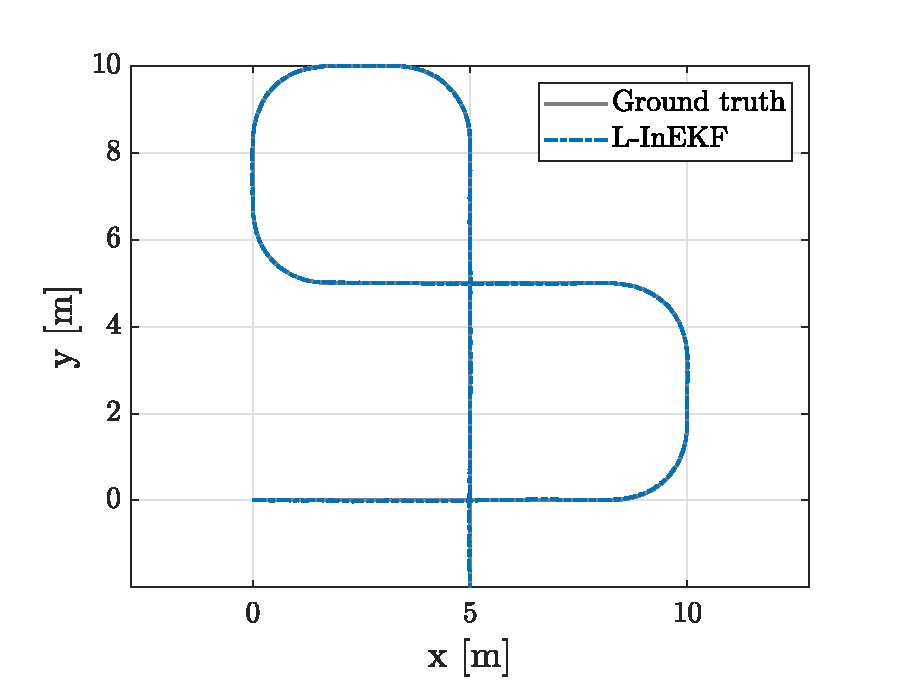
\includegraphics[width=\textwidth]{figs/se2_example_trajectories.eps}
        \caption{Ground truth and estimated trajectories from the $SE(2)$ example.}
        \label{fig:se2_example_trajectories}
    \end{figure}

    \begin{figure}[h]
        \centering
        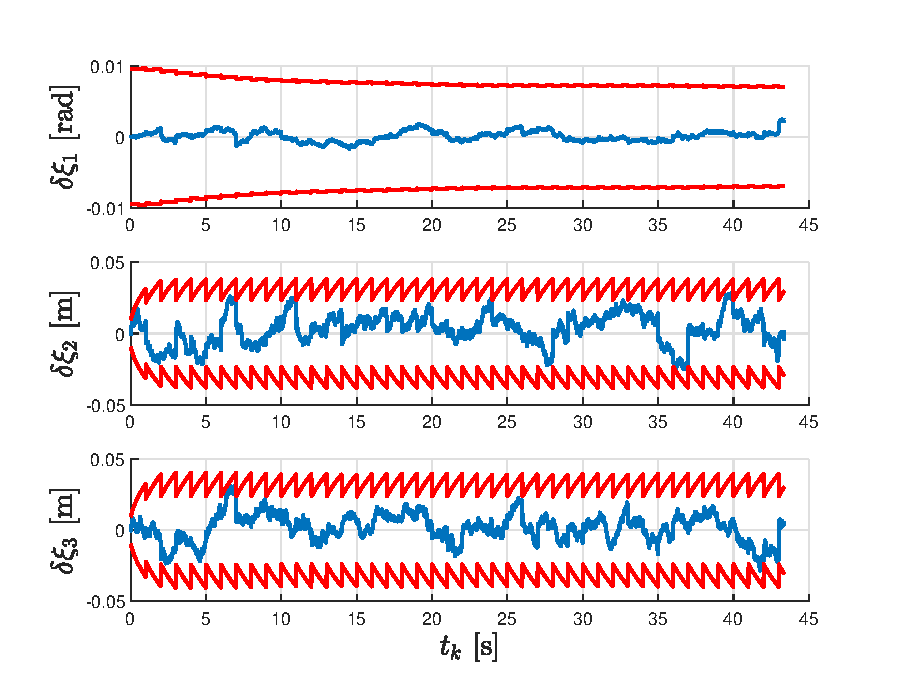
\includegraphics[width=\textwidth]{figs/se2_example_error_plots.eps}
        \caption{Error plots from the $SE(2)$ example.\\ Note that $\mbs{\xi}_{k} = \Log(\mbf{X}_{k})$, where $\mbf{X}\in SE(2)$ is the $SE(2)$ pose at time $t_{k}$.}
        \label{fig:se2_example_error_plots}
    \end{figure}


    \clearpage
    % \backmatter
    \bibliography{references}
    % \bibliographystyle{plainnat}
    \bibliographystyle{IEEEtran}
\end{document}